\section{Aufbau}\label{sec:aufbau}

In der Abbildung \ref{fig:aufbau} ist die zusammengebaute Yagi-Uda-Antenne dargestellt. Die wichtigsten Bestandteile der Antenne sind die 3D-Elemente, die Aluminiumstäbe, das Rundholz und die Speisung des Dipols. Alle benötigten Bauteile sind in der Tabelle \ref*{tab:materialliste} aufgeführt. Jedes dieser Bestandteilen ist mit einer Nummer versehen, welche sich in der Abbildung beim passenden Element befindet. Die 3D-Elemente und der Aufbau des Dipols werden später noch genauer erklärt.

\begin{figure}[H]
	\centering
	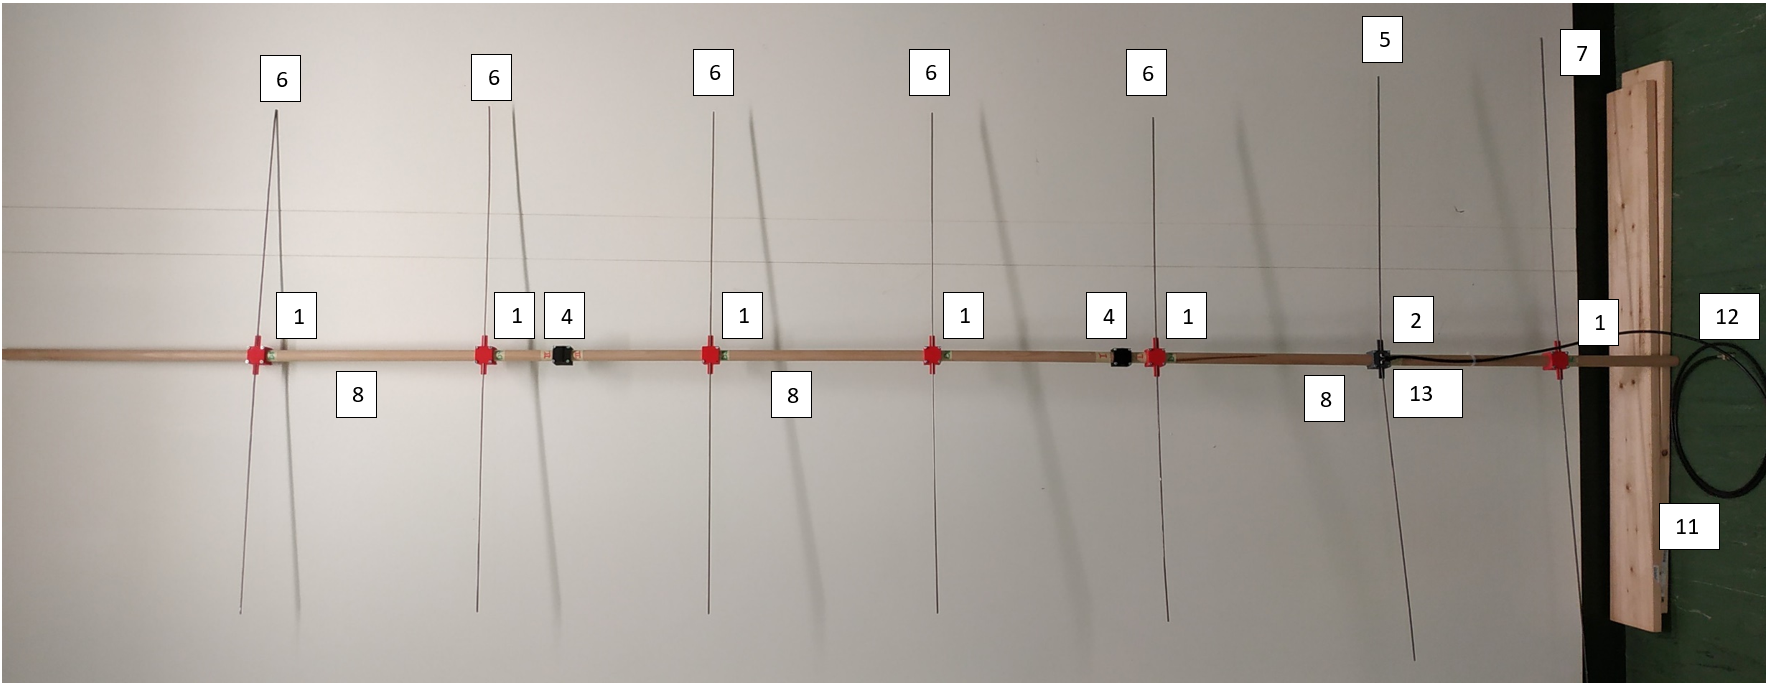
\includegraphics[width=0.9\linewidth]{aufbau}
	\caption{Aufbau eigener Yagi-Antenne mit nummerierten Bauteilen}\label{fig:aufbau}
\end{figure}

\begin{table}[H]
	\centering
	\begin{tabular}{>{\tt}C{1.7cm}| L{6.5cm}| L{3.6cm}| C{1.5cm}} 
		\normalfont\textbf{Nummer} & \normalfont\textbf{Bauteil} & \normalfont\textbf{Hersteller} & \normalfont\textbf{Anzahl} \\ \hline\hline 
		1	&	3D-Element Direktor/Reflektor 	& Eigenkonstruktion	& 6    \\ \hline
		2	&	3D-Element Dipol 				& Eigenkonstruktion	& 1    \\ \hline
		3	&	3D-Element Unten 				& Eigenkonstruktion	& 7    \\ \hline
		4	&	3D-Element Halterung 			& Eigenkonstruktion	& 2    \\ \hline
		5	&	Aluminiumstab $\oslash \SI{2}{mm}$ Dipol 			& FHNW Werkstat		& 1    \\ \hline
		6	&	Aluminiumstab $\oslash \SI{2}{mm}$ Direktor 		& FHNW Werkstat		& 5    \\ \hline
		7	&	Aluminiumstab $\oslash \SI{2}{mm}$ Reflektor 		& FHNW Werkstat 	& 1    \\ \hline
		8	&	Holzrundstab  $\oslash \SI{20}{mm}$, L=$\SI{1}{m}$					& Jumbo			 	& 3    \\ \hline
		9	&	M3 Impusschrauben  				& Institut ISE		& 36    \\ \hline
		10	&	M3 Mutern  						& Institut ISE 		& 36    \\ \hline
		11	&	Kabel 							& Institut ISE 		& 1    \\ \hline
		12	&	Stecker	  						& Institut ISE 		& 1    \\ \hline
		13	&	Kabelschuh	  					& Institut EA		& 2    \\ \hline
	\end{tabular}
	\caption{Zusammenstellung aller verwendeten Bauteilen.}
	\label{tab:materialliste}
\end{table}

Die Halterung für den Dipol, den Reflektor und die Direktoren sind mit einem 3D-Drucker hergestellt worden. Die Zeichnungen sind im Autodesk Fusion 360 konstruiert worden und danach mit dem Ultimaker 2+ gedruckt. Die Elemente sind in der Abbildung \ref*{fig:3D-Elemente} dargestellt.\\

Das spezielle der Konstruktion für die Halterung für den Dipol (Bild a) ist, dass sie Platz bietet um das Koaxialkabel anzuschliessen sowie die beiden Aluminiumstäbe, welche den Dipol bilden in der Mitte trennt.\\
Die Halterung für den Direktor/Reflektor (Bild b) ist so konstruiert, dass der Aluminiumstab sehr einfach durch die Öffnung hindurchgeschoben und mit Leim fixiert werden kann. \\
Mit dem Gegenstück der Halterung (Bild c), vier Impusschrauben und dem Oberteil (Bild a,b) kann das Element auf dem Trägerstab montiert werden. Die drei Trägerstäbe werden mit zwei Gegenstücke zusammengebaut. Nun können die Distanzen zwischen den Elementen ganz einfach angepasst werden durch leichtes lösen der Schrauben.

\begin{figure}[H]
	\centering
	\subfloat[Halterung für den Dipol]{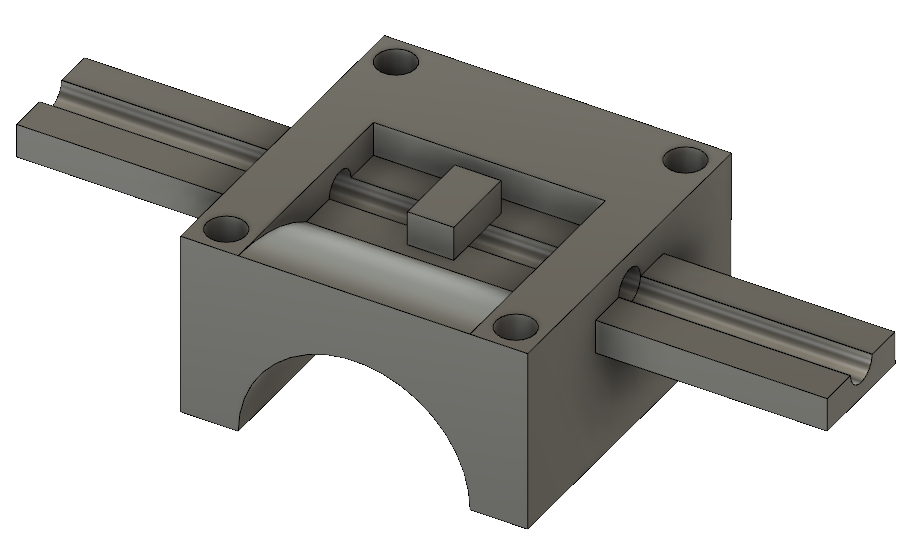
\includegraphics[width=0.4\linewidth]{oben_dipol}}\qquad
	\subfloat[Halterung für die parasitären Element]{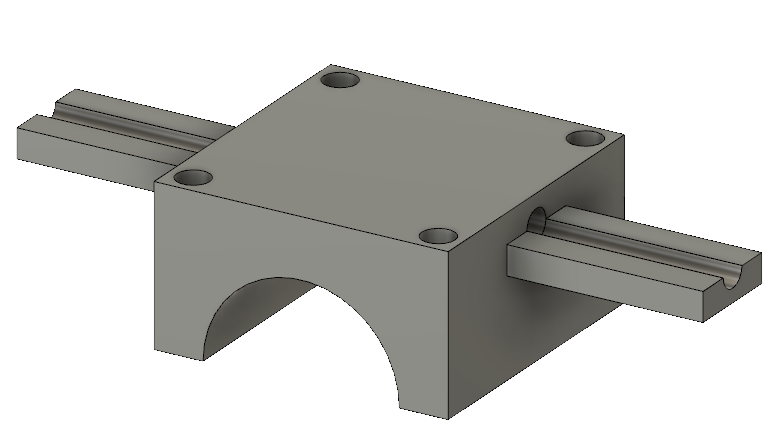
\includegraphics[width=0.4\linewidth]{oben_direktor}}\qquad
	\subfloat[Gegenstück der Halterungen]{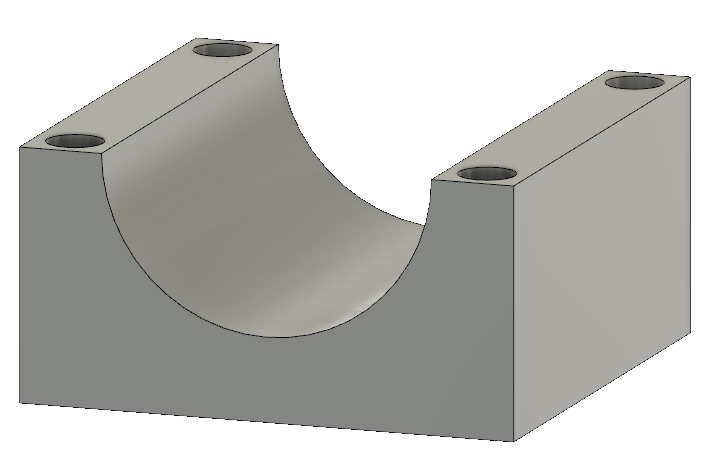
\includegraphics[width=0.3\linewidth]{unten}}
	\caption{Zeichnungen der 3D-gedruckten Elemente }
	\label{fig:3D-Elemente}
\end{figure}

In der Abbildung \ref*{fig:aufbau_dipol} ist der Aufbau des Dipols dargestellt. Der Leiter des Koaxialkabels ist am einten Teil und er Schirm an dem anderen Teil des Diplos angebracht. Die Befestigung wurde mit einem Kabelschuh realisiert. Dafür wurde bei dem Aluminiumstab ein Aussengewinde gedreht. Zum Schutz wurde das ganze mit einem Schrumpfschlauch versehen.

\begin{figure}[H]
	\centering
	\includegraphics[width=0.45\linewidth]{dipol}
	\caption{Aufbau des Dipols der Yagi-Antenne}\label{fig:aufbau_dipol}
\end{figure}





